%! TEX root = ../main.tex

\documentclass[../main.tex]{subfiles}

\begin{document}
\chapter{July 8th to July 13th, 2025}
Second meeting with Dr Amato.
\section{Meeting Minutes}
\subsection{Quick notes}
\begin{itemize}
    \item Dr Amato seemed happy with my progress.
    \item He will give me access to 227 and update me on the risk assessments, I had to give him my RAFT form.
    \item Explained how mount models work: Input desired positions then platesolves for actual position. Many points creates a spherical surface of the errors.
    \item Assembly as soon as possible.
    \item New project: Programmatic control of the mount. Start by following a predetermined path, closed loop control is the end goal.
    \item Need to book Blackett roof for observations, but for now use the open area in floor 3 next to his room.
    \item Model Creator was just not maximised!! I reinstalled ASCOM 7, 6.6, Mount Creator, .NET frameworks and everything, I was so stupid!!
\end{itemize}
\section{Quick notes}
\begin{itemize}
    \item PyPOGS might not be usable with 10Micron mount, I will be using ASCOM python interface for now. The \href{https://ascom-standards.org/Help/Developer/html/T_ASCOM_DeviceInterface_ITelescopeV3.htm}{ ITelescopeV3 interface} has all the functions I need.
    \item Mount Creator is maintained and can be run on command line for automatic control. However, it seems everyone uses \href{https://mworion.github.io/MountWizzard4/}{Mount Wizzard 4} for mount calbration so I will look into it.
    \item Dr Amato suggested using the mount without telescope/weight attached, I don't think that is a good idea
    \item Sent: Is it safe to motorise (skew) the AZ1000HPS ALTAZIMUTH MOUNT axes without putting the telescope and the counterweight on? I want to try testing slewing over the ASCOM protocol with Python safely, without all the heavy weight on the mount, which might cause expensive damage. To \href{https://10micron.eu/en/contact}{their contact page}. I also posted the question to the \href{https://www.10micron.com/forum/viewtopic.php?f=2&t=2283}{10Micron forum}.
    \item UPDATE: \href{https://www.10micron.com/forum/viewtopic.php?f=2&t=2283&p=19410#p19410}{They replied} saying it is safe to do that! Especially for the Alt/Az mounts. Technical support also replied: Dear Mr. Leung, yes, it is safe to slew the mount without any load like telescope, counterweight a.s.o. Best regards Michael Risch.
    \item MountWizzard4 has \href{https://www.youtube.com/@orion49m/videos}{video tutorials}.
    \item MountWizzard4 is kind of annoying, for now if I want to run it use run.bat as it requires Python 3.10 and I have 3.11 installed natively.
    \item Using the ASCOM OMNI-simulator and win32com works, it just simply works.
    \item Possibly will use ASTAP from now on for plate solving.
\end{itemize}
\begin{itemize}
    \item Inputs: Dense path over time of the TLE propagated trajectory
    \item Outputs: Axis rates and positions / Slewing?
    \item look at how PyPOGS moves the mount, does it slew or follow rates
    \item Make sure the control system is documented well
    \item SATchecker
\end{itemize}
\subsection{Notes on ASCOM interface:}
\begin{itemize}
    \item \href{https://ascom-standards.org/Help/Developer/html/T_ASCOM_DeviceInterface_ITelescopeV3.htm}{ITelescopeV3} interface has most of what I am going to talk about, but here are a quick few notes:
    \item SlewToAltAzAsync and SlewToCoordinatesAsync (RA/DEC) for going to a position.
    \item AltAz must have tracking disabled \verb|mount.Tracking = False| to slew, and for Coordinates it must be enabled \verb|mount.Tracking = True| to slew or else will return an error.
    \item Non Async versions return after the slew is complete, so pretty useless for path tracking.
    \item I thought I would be able to use TargetDeclination or TargetRightAscention, which according to the documentation should be updated when SlewToCoordinates(Async) is called, but for the omnisim, not sure if this is true for the real mount the target equals the current position while slewing, so it is useless?
    \item Slew speed is set by the mount, which for 10Micron can be set in the driver when the driver is initialised. More details on the driver notes \cref{fig:10microndriver_drive}
    \item The omnisim slewing seems to move in weird directions when slewing? Maybe this will change on the 10micron mounts. I can safely test without the telescope or counterweight attached according to the forums and technical support.
    \item Will now try to develop a open loop (derivatives of axis rates from any designated path, later on being TLE trajectory) then closed loop to bring it closer using \verb|MoveAxis(0, 1)| and \verb|MoveAxis(1, 1)|, where 0 is primary axis  (e.g., Right Ascension or Azimuth), and 1 is secondary axis  (e.g., Declination or Altitude) according to the documentation.
    \item Maybe use \verb|SetPark()| and \verb|Unpark()| when stopped to be safe. Also, use guard statements and logging with all the "Can" commands to check if the mount is ready to move, e.g., \verb|CanMoveAxis(0)| and \verb|CanSlew|. Also, use \verb|IsSlewing| to check if the mount is currently moving.
\end{itemize}
\subsection{Notes on driver}
\begin{itemize}
    \item Driver is only available \href{https://www.10micron.com/forum/viewtopic.php?f=3&t=1907}{on the forums} with a verified account (using the mount serial number).
    \item Slew settings on drive \cref{fig:10microndriver_drive} in deg/s, according to Dr Amato max 15deg/s but I read never above 10 on the manual?
    \item Must select Enable sync \cref{fig:10microndriver_sync} when using model creator! That is the whole point of model creator!!
    \item Here are some pictures:
\end{itemize}
\begin{figure}[h]
    \centering
    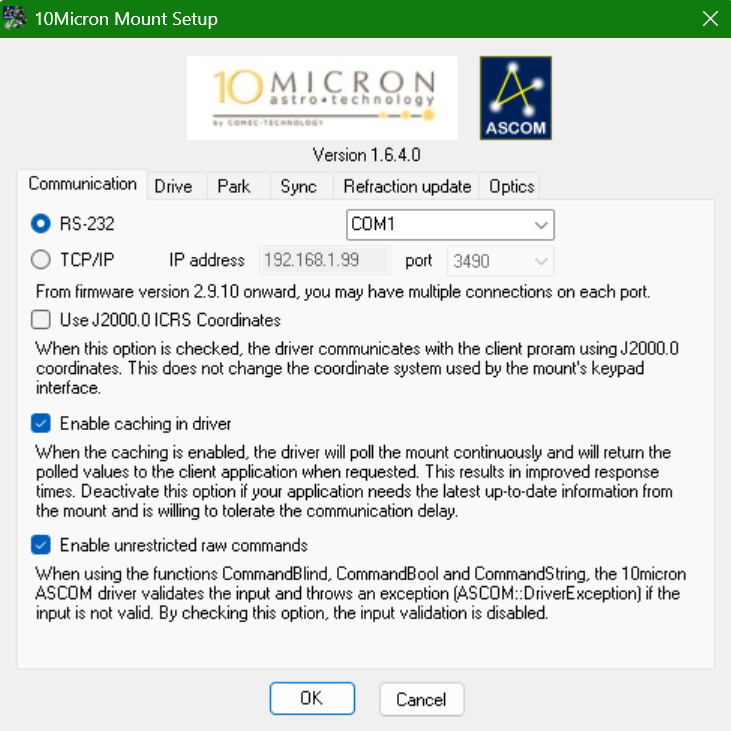
\includegraphics[width=0.5\textwidth]{10microndriver1.png}
    \caption{Main screen of the 10Micron driver.}
    \label{fig:10microndriver1}
\end{figure}
\begin{figure}[h]
    \centering
    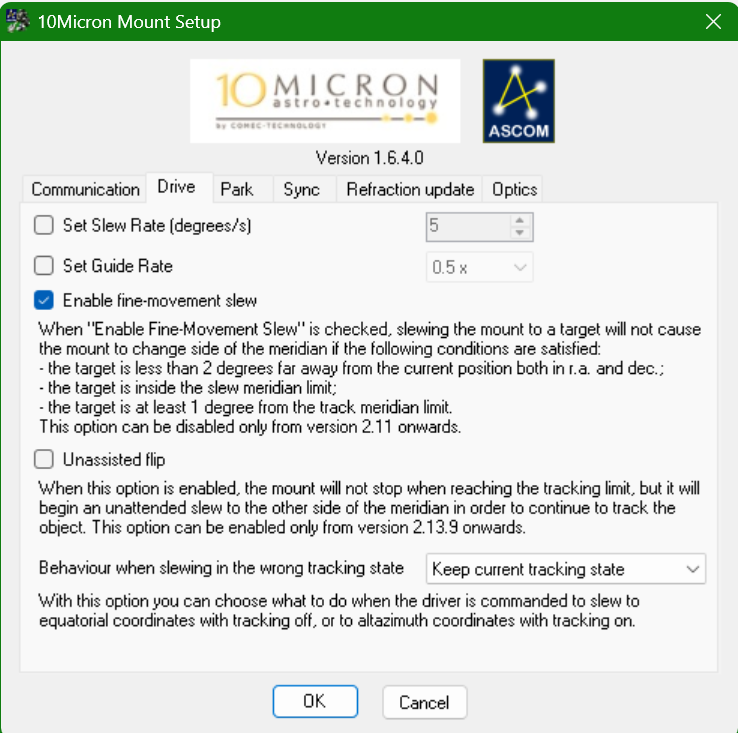
\includegraphics[width=0.5\textwidth]{10microndriver2.png}
    \caption{Drive settings of the 10Micron driver.}
    \label{fig:10microndriver_drive}
\end{figure}
\begin{figure}[h]
    \centering
    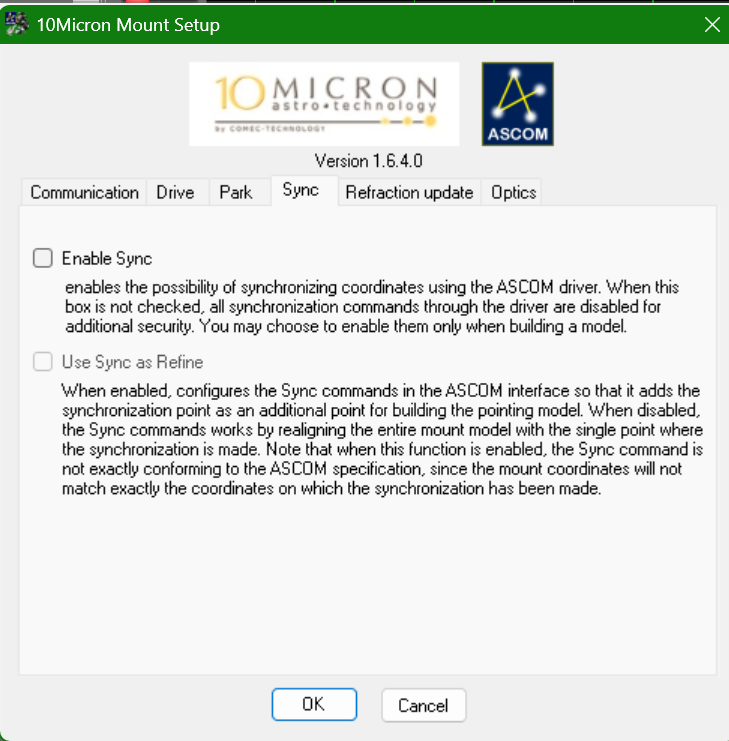
\includegraphics[width=0.5\textwidth]{10microndriver3.png}
    \caption{Sync settings of the 10Micron driver.}
    \label{fig:10microndriver_sync}
\end{figure}
\subsection{SATchecker}
\begin{itemize}
    \item This is hell. Their setup process doesn't work. I have raised an \href{https://github.com/iausathub/satchecker/issues/157}{issue on the github} and will try to get it working.
    \item Here are the steps by steps of how to install it that I know for windows. Modified version of \href{https://github.com/iausathub/satchecker/wiki/setup}{this setup} as that doesn't work.: \begin{enumerate}
        \item \verb|git clone https://github.com/iausathub/satchecker.git|
        \item \verb|python3 -m venv venv|
        \item \verb|venv/Scripts/activate|
        \item \verb|cd src/api|
        \item \verb|pip install -r requirements.txt|
        \item Now, the setup says to run the API server but that doesn't work yet.
        \item In \verb|.flaskenv| change \verb|LOCAL_DB=0| to \verb|LOCAL_DB=1|
        \item Install Docker Desktop for your OS: \href{https://www.docker.com/products/docker-desktop}{here}
        \item Cd in terminal to \verb|dev/local_db|
        \item \verb|docker build -t satchecker-db .|
        \item \verb|docker volume create satchecker_db_vol|
        \item \lstinline{docker run -d --name satchecker-db -v satchecker_db_vol:/var/lib/postgresql/data -p 5432:5432 satchecker-db} 
        \item Go to \verb|src/api| and run the following commands to retrieve TLEs:
        \item \lstinline{python retrieve_TLE.py -m gp -s localhost -p 5432 -d postgres -u postgres -pw sat123 -sc celestrak}
        \item \lstinline{python retrieve_TLE.py -m sup -s localhost -p 5432 -d postgres -u postgres -pw sat123 -sc celestrak}
        \item Download redis from \href{https://github.com/tporadowski/redis/releases}{here} through the installer
        \item In one terminal instance (I was using powershell) run \verb|$env:PYTHONPATH = "C:\...Yourpath...\satchecker\src"|
        \item Then run \verb|flask run| 
    \end{enumerate}
    \item This should put all the TLEs in the database, but the flask server doesnt show any! Apparently all the launch dates and decay dates are required to be in the database, but they don't exist from the TLEs! The github issue might fix that.
    \item Use \href{https://www.pgadmin.org/}{pgAdmin} to connect to the database and check if the TLEs are there
\end{itemize}
\subsection{MountWizzard4}
\begin{itemize}
    \item This seems a bit too complicated to get working, but I had it installed.
    \item ONLY works on python 3.8-3.10, it can only be ran like that! The only way I got it to install was through this github \href{https://github.com/mworion/InstallerMW4/releases}{release page} and this \href{https://www.youtube.com/watch?v=Tzob8ZSnMH0}{youtube video}.
    \item Obviously use python10.exe instead of python for the video.
    \end{itemize}

    Amato Notes
    \begin{itemize}
        \item Moon and stars in the sky chart - Helpful for visual observation, magnitude 2
        \item Satchecker might be nice to contribute to open source
        \item Automate satchecker, spacetrack
        \item CICLOPS Control github repo on COAST
        \item Fork satchecker to COAST with our own branch
        \item Pay attention when I handle it because there are clutches. When the clutches are tightened, the mount is engaged, the motor is engaged to the axis, when the clutch is disengaged the motor is not engaged. When I handle the mount I must have the clutch disengaged.
        \item Go to room 309 and ask biruk to help.
        \item 
\end{itemize}
SATCHECKER WORKING!!!
\begin{itemize}
    \item \begin{lstlisting}
        http://localhost:5000/ephemeris/name-jdstep/?name=ISS%20(ZARYA)&latitude=51.4915&longitude=-0.2073&elevation=222&startjd=2460871&stopjd=2460872&stepjd=0.01
    \end{lstlisting}
\end{itemize}
\end{document}